\documentclass[15pt, a4paper]{article}
\usepackage[T1]{fontenc}
\usepackage[polish]{babel}
\usepackage[utf8]{inputenc}
\usepackage{tikz}
\usepackage{adjustbox}
\usepackage{longtable}
\usepackage{graphicx}
\title{Obliczenia naukowe}
\author{Felix Zieliński 272336}
\date{Lista 2}
\begin{document}
\maketitle
TODO OPIS, czy zadanie 2?

\vspace{0.5cm}

\noindent\hrulefill

% zadanie 1

\vspace{0.5cm}

\noindent\textbf{Zadanie 1.} Niewielkie zmiany danych oraz ich wpływ na wyniki obliczeń.\\

\noindent W ramach przypomnienia zadania: na poprzedniej liście  należało obliczyć iloczyny skalarne dwóch wektorów na cztery rózne sposoby.\\\\
Zaimplementowałem każdy z podanych w poleceniu sposobów, tak więc funkcja \verb|a| liczy "w przód", od pierwszych indeksów, funkcja \verb|b| "w tył", analogicznie, a \verb|c| oraz \verb|d| liczą, odpowiednio, od największego do najmniejszego oraz od najmniejszego do największego względem ich wartości absolutnej.\\\\
Różnica w tym zadaniu, a zadaniu 5. z poprzedniej listy polegała na dokonaniu drobnej zmiany w niektórych wartościach wektora. Poniżej prezentuję wyniki otrzymane po, jak i przed tej zmianie:


\begin{table}[ht]
    \begin{adjustbox}{max width=\textwidth}
    \begin{tabular}{|c|c|c|c|c|}
        \hline 
        Sposób & Float32 stare & Float32 nowe & Float64 stare & Float64 nowe \\ \hline
        a & -0.4999443 & -0.4999443 & 1.0251881368296672e-10 & -0.004296342739891585 \\ \hline
        b & -0.4543457 & -0.4543457 & -1.5643308870494366e-10 & -0.004296342998713953 \\ \hline
        c & -0.5 & -0.5 & 0.0 & -0.004296342842280865 \\ \hline
        d & -0.5 & -0.5 & 0.0 & -0.004296342842280865 \\ \hline
    \end{tabular}
    \end{adjustbox}
    \caption{Porównanie nowych i starych danych}
    \label{tab:products}
\end{table}

\vspace{0.5cm}

\noindent gdzie wartość prawidłowa wynosi: \[\verb|-1.00657107000000e-11|\]

Jak widać, wyniki dla typu \verb|Float32| nie zmieniły się. Jest to spowodowane niewystarczającą do zauważenia różnicy precyzją zapisu liczby zmiennopozycyjnej w tym typie.\\\\
Natomiast w typie \verb|Float64| różnica jest znaczna mimo tak niewielkiej zmiany danych. Mimo że wyniki nadal odbiegają od prawidłowego, są one mu znacznie bliższe. \\\\
Można więc stwierdzić, że zadanie to było \textbf{źle uwarunkowane} - o wysokim wskaźniku uwarunkowania. Wskaźnik ten określa, w jakim stopniu błąd reprezentacji numerycznej danych wejściowych dla danego problemu będzie wpływać na błąd wyniku. Małe zmany danych w tym zadaniu spowodowały znaczną zmianę wyników. 

\vspace{0.5cm}

\noindent\hrulefill

% zadanie 2

\vspace{0.5cm}

\noindent\textbf{Zadanie 2.} W tym zadaniu należało narysować wykres funkcji \[f(x) = e^{x}\ln(1 + e^{-x})\] 
w dwóch różnych programach do wizualizacji danych. Zdecydowałem się na użycie WolframaAlpha, Desmosa oraz Gnuplota

\begin{figure}[h]
    \centering
    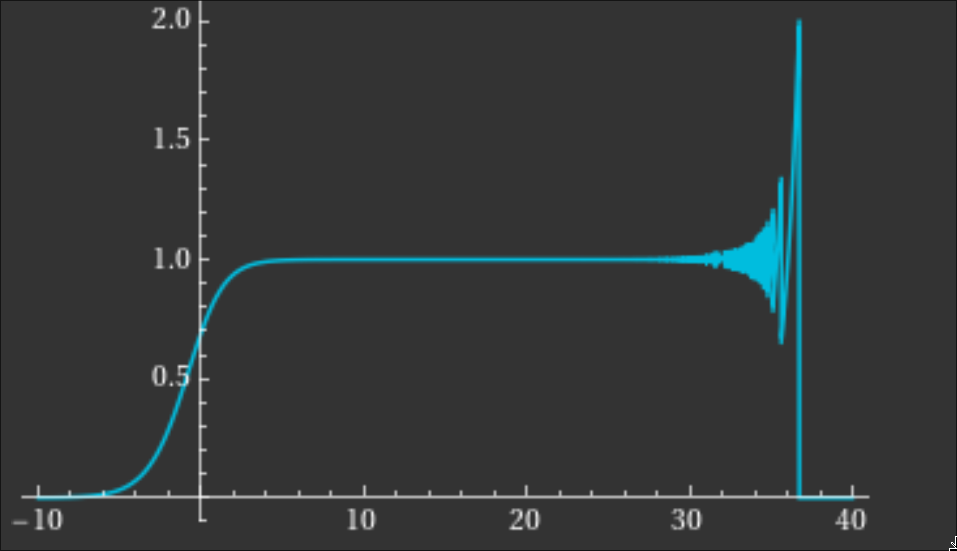
\includegraphics[width=0.5\textwidth]{img/wolfram1.png}  
    \caption{WolframAlpha: \texttt{plot $e^{x} * \ln(1 + e^{-x})$ from $x = -10$ to $x = 40$}}
\end{figure}

\begin{figure}[h]
    \centering
    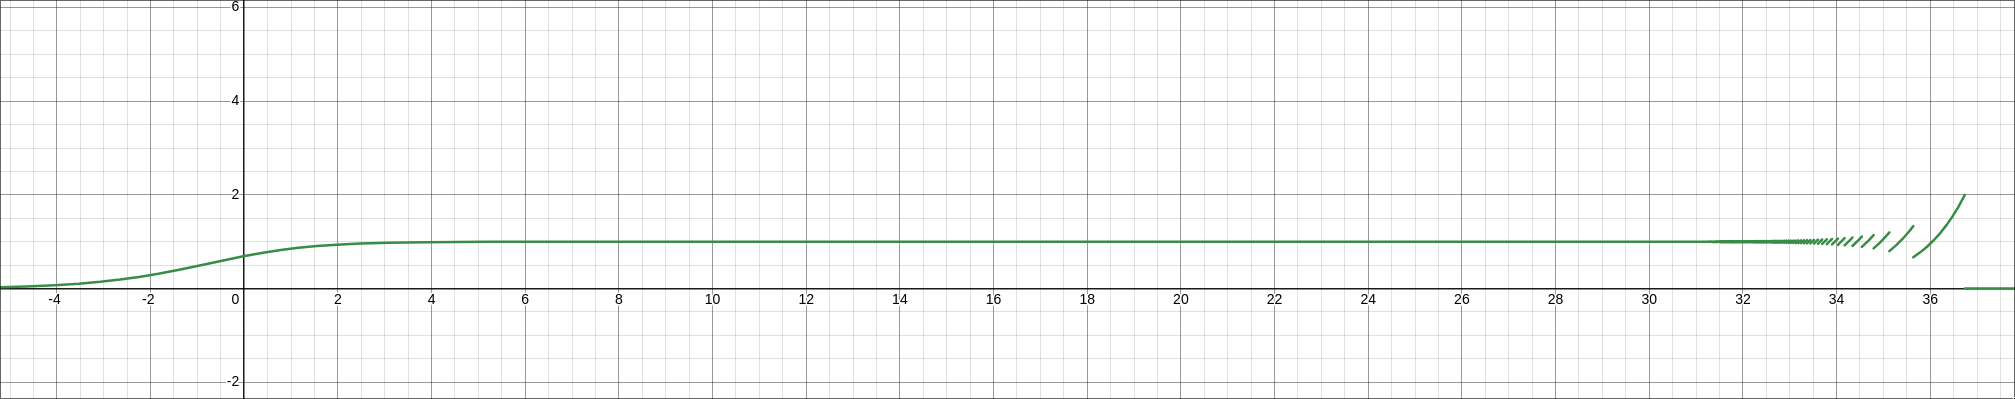
\includegraphics[width=0.5\textwidth]{img/desmos1.png}
    \caption{Desmos}
\end{figure}

\begin{figure}[h]
    \centering
    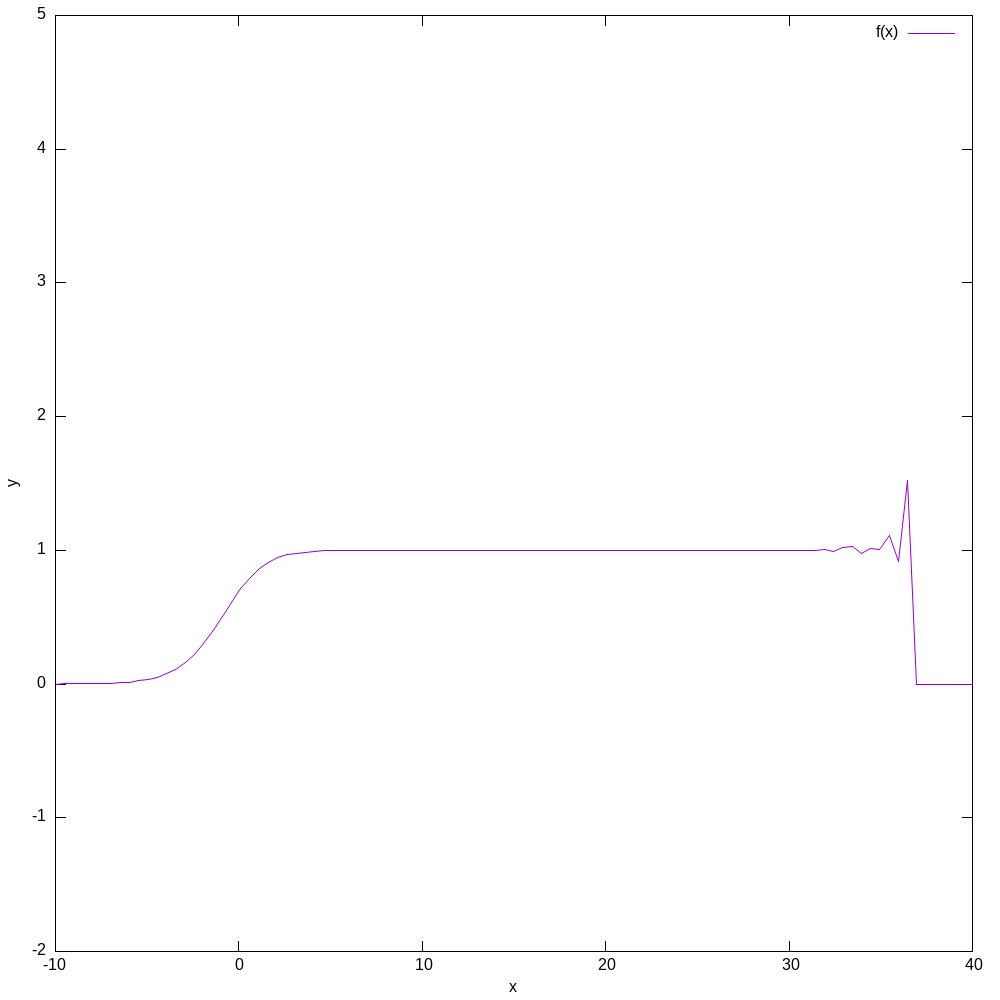
\includegraphics[width=0.5\textwidth]{img/gnuplot1.png}
    \caption{Gnuplot}
\end{figure}

\vspace{0.5cm}

\noindent Granica tej funkcji dla x zmierzającego do nieskończoności wynosi 

\[
\lim_{x \to \infty} f(x) = \lim_{x \to \infty} e^x \ln(1 + e^{-x}) = 1
\]

\noindent Jak można zauważyć, dla wartości \verb|x >\ 32| wykresy zaczynają wskazywać błędne wartości, każdy na trochę inny sposób. Oscylują one wokół 1, coraz bardziej odbiegając od jej wartości, a następnie spadają do 0. \\\\

\noindent Dzieje się tak, gdyż dla \verb|x > 30| wartości $e^{x}$ są już tak duże, że mnożenie jej z niewielką wartością $ln(1 + e^{-x})$ skutkuje znacznymi błędami przybliżenia, które dla ok \verb|x = 38| powodują zwracanie wartości 0. Jest to spowodowane przybliżeniem $1 + e^{-x} \approx 1$, i tym samym całej wartości logarytmu do 0. Tak więc algorytm obliczający wartości \verb|f(x)| nie jest stabilny numerycznie.

\vspace{0.5cm}

\noindent\hrulefill

% zadanie 3

\vspace{0.5cm}









\end{document}
